\section{Testing and Results}
\subsection{Testing Method}
To test the system, a generated set of module configurations were input into the system, and the total time spent in the logic layer and hardware layer were recorded separately for both the system with and without physical constraints applied. An average time is then calculated for configurations consisting of 4 – 9 modules. The branching factor was also varied throughout the test to analyse the effect on total time, failure rate and number of moves returned in the final solution.

\subsection{Performance Metric}
To measure performance of the overall system, the testing methods measure:
\begin{itemize}[]
	\item The number of failures encountered during the solution search with feedback strategies.
	\item The number of modules effect on failure count
	\item The number of search branches effect on failure count
	\item The number of search branches effect on number of moves in the solution.
	\item The number of search branches effect on search time.
	\item Total calculation time.
\end{itemize}
To quantify the performance of the implemented feedback strategy, the number of semantic solutions that fail in the physical layer is used. The physical layer is the most computationally demanding section of the overall system, so it should be used as little as possible. Time spent calculating results is recorded for comparison with other systems and to prove the systems capabilities for real-world use but is not considered a measure of project success.

\subsection{Analysis of Results}
\begin{figure}[H]
	\centering
	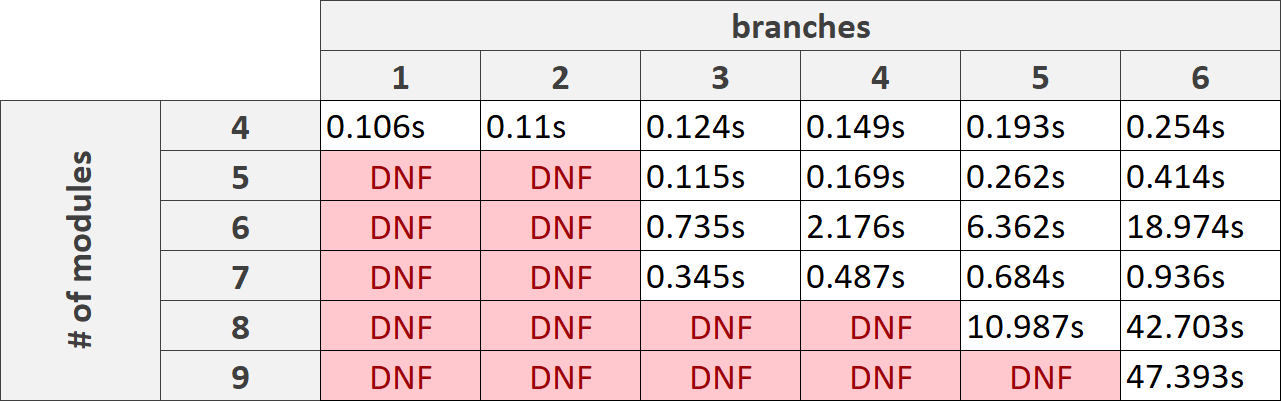
\includegraphics[width=\textwidth]{avgMoveTime.png}
	\caption{Average time per move to find a solution}
	\label{avgMoveSol}
\end{figure}
Tests were conducted on a system with the hardware specifications shown in section \ref{hardware}, results can be seen in \nameref{testResultsSec}. As expected, as the number of modules in the input configuration rises, so does the number of physical layer failures during the solution search as fig \ref{failures} shows. Interestingly, the more modules in the state, the higher the number of branches the task planner is using needs to be to completely avoid failing the search by reaching max recursions. Fig \ref{avgMoveSol} shows a good example of this where failed tests are labelled DNF, and passed tests show the total time take to find a solution divided by the number of moves in the solution, giving an average time per generated move. The time it takes to find a solution seems to be almost completely irrelevant for analysis of the system, as it is dependent on the configuration of the state entered. For example, if a module must be moved out of its final position first to enable another module to be moved to its final position, it will take longer to find a solution than if all modules are already accessible.
\\\\
\begin{figure}[H]
	\centering
	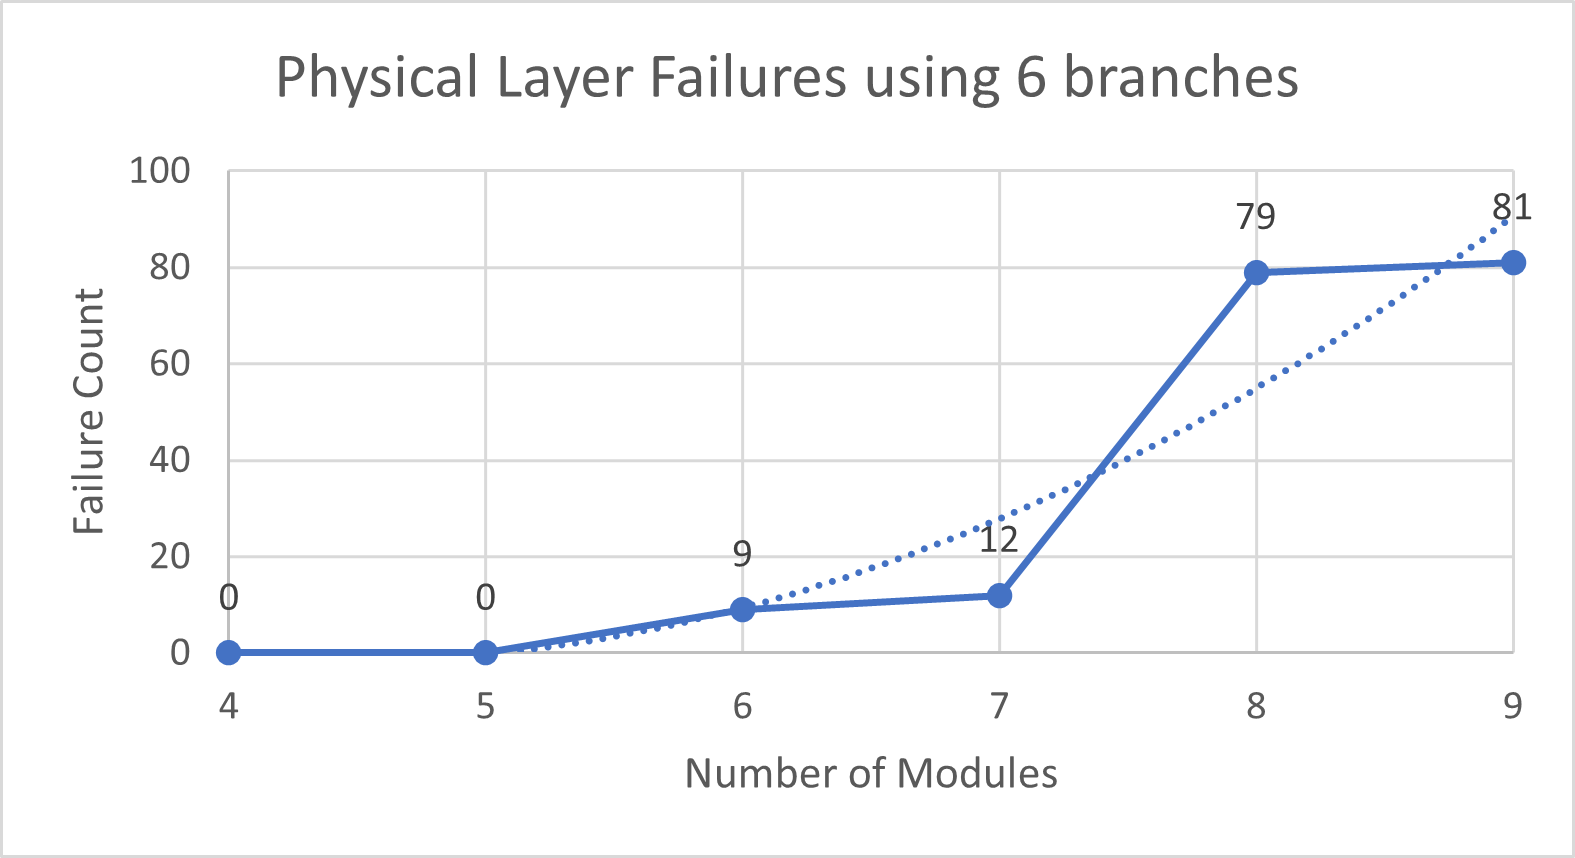
\includegraphics[width=0.9\textwidth]{failures.png}
	\caption{Failures vs Number of Modules for solutions found using 6 branches}
	\label{failures}
\end{figure}
\begin{figure}[H]
	\centering
	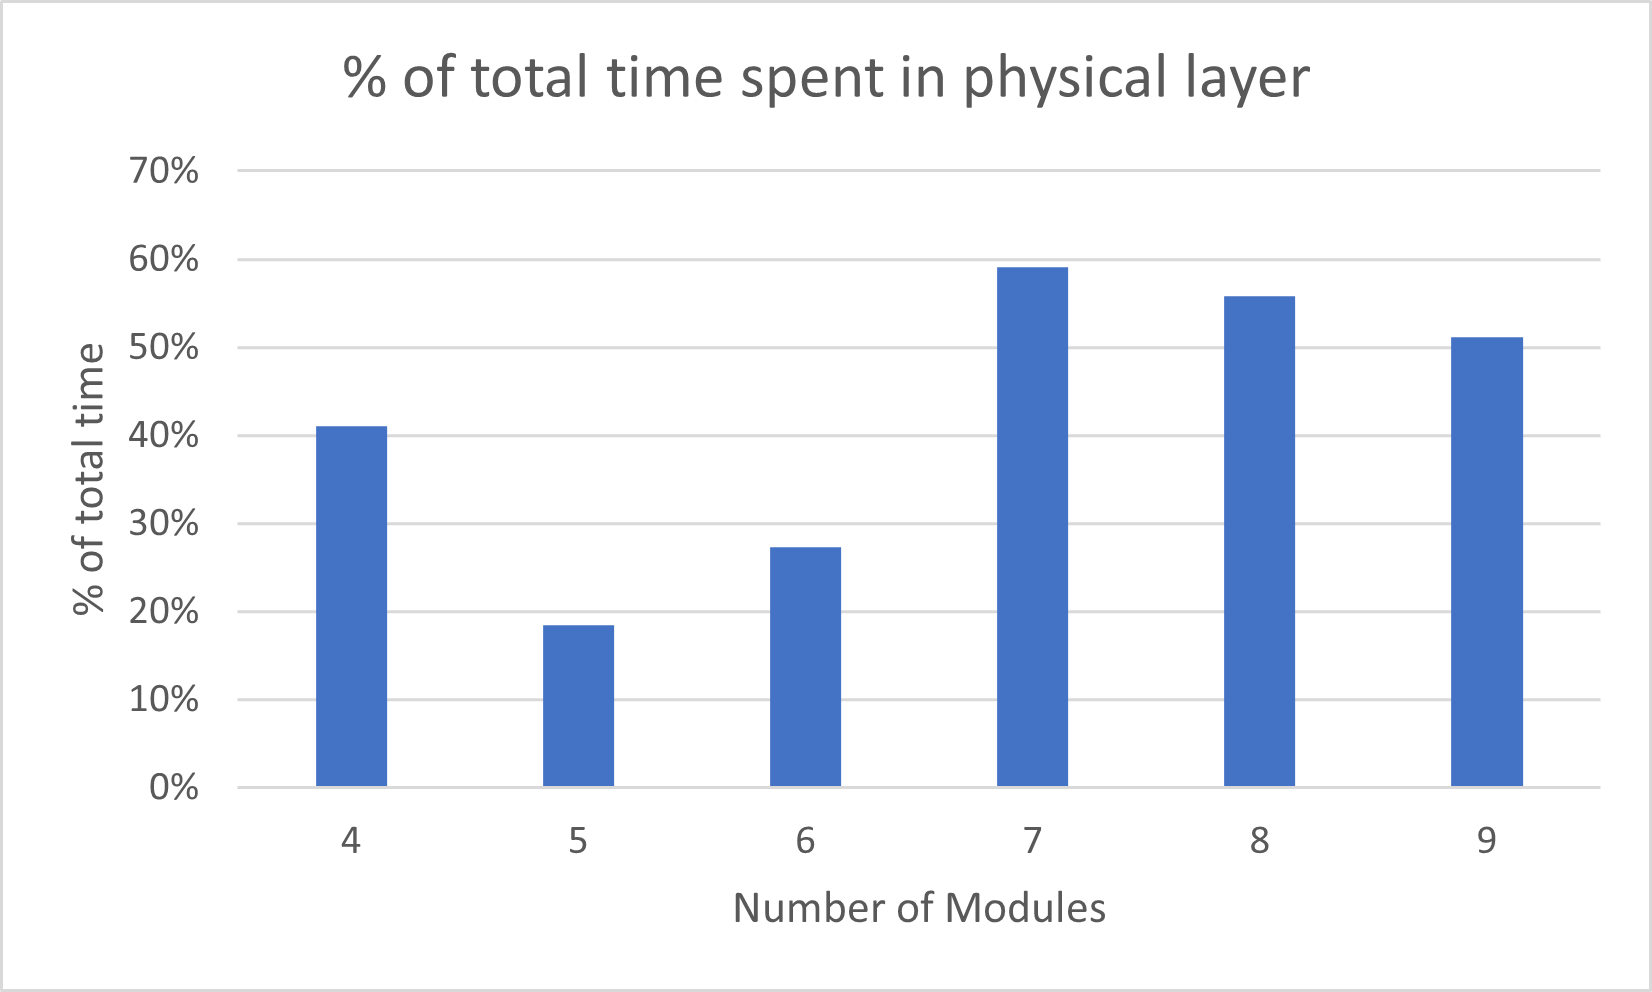
\includegraphics[width=0.9\textwidth]{physicaltime.png}
	\caption{Percent of total time spent in the physical layer to find a solution (on average)}
	\label{physicalLayerTime}
\end{figure}